% This is "sig-alternate.tex" V1.9 April 2009
% This file should be compiled with V2.4 of "sig-alternate.cls" April 2009
%
% This example file demonstrates the use of the 'sig-alternate.cls'
% V2.4 LaTeX2e document class file. It is for those submitting
% articles to ACM Conference Proceedings WHO DO NOT WISH TO
% STRICTLY ADHERE TO THE SIGS (PUBS-BOARD-ENDORSED) STYLE.
% The 'sig-alternate.cls' file will produce a similar-looking,
% albeit, 'tighter' paper resulting in, invariably, fewer pages.
%
% ----------------------------------------------------------------------------------------------------------------
% This .tex file (and associated .cls V2.4) produces:
%       1) The Permission Statement
%       2) The Conference (location) Info information
%       3) The Copyright Line with ACM data
%       4) NO page numbers
%
% as against the acm_proc_article-sp.cls file which
% DOES NOT produce 1) thru' 3) above.
%
% Using 'sig-alternate.cls' you have control, however, from within
% the source .tex file, over both the CopyrightYear
% (defaulted to 200X) and the ACM Copyright Data
% (defaulted to X-XXXXX-XX-X/XX/XX).
% e.g.
%\CopyrightYear{2009} will cause 2007 to appear in the copyright line.
% \crdata{0-12345-67-8/90/12} will cause 0-12345-67-8/90/12 to appear in the copyright line.
%
% ---------------------------------------------------------------------------------------------------------------
% This .tex source is an example which *does* use
% the .bib file (from which the .bbl file % is produced).
% REMEMBER HOWEVER: After having produced the .bbl file,
% and prior to final submission, you *NEED* to 'insert'
% your .bbl file into your source .tex file so as to provide
% ONE 'self-contained' source file.
%
% ================= IF YOU HAVE QUESTIONS =======================
% Questions regarding the SIGS styles, SIGS policies and
% procedures, Conferences etc. should be sent to
% Adrienne Griscti (griscti@acm.org)
%
% Technical questions _only_ to
% Gerald Murray (murray@hq.acm.org)
% ===============================================================
%
% For tracking purposes - this is V1.9 - April 2009

\documentclass{sig-alternate}

\begin{document}
%
% --- Author Metadata here ---
%\conferenceinfo{WOODSTOCK}{'97 El Paso, Texas USA}
%\CopyrightYear{2007} % Allows default copyright year (200X) to be over-ridden - IF NEED BE.
%\crdata{0-12345-67-8/90/01}  % Allows default copyright data (0-89791-88-6/97/05) to be over-ridden - IF NEED BE.
% --- End of Author Metadata ---

\title{Unified Execution Model}
%
% You need the command \numberofauthors to handle the 'placement
% and alignment' of the authors beneath the title.
%
% For aesthetic reasons, we recommend 'three authors at a time'
% i.e. three 'name/affiliation blocks' be placed beneath the title.
%
% NOTE: You are NOT restricted in how many 'rows' of
% "name/affiliations" may appear. We just ask that you restrict
% the number of 'columns' to three.
%
% Because of the available 'opening page real-estate'
% we ask you to refrain from putting more than six authors
% (two rows with three columns) beneath the article title.
% More than six makes the first-page appear very cluttered indeed.
%
% Use the \alignauthor commands to handle the names
% and affiliations for an 'aesthetic maximum' of six authors.
% Add names, affiliations, addresses for
% the seventh etc. author(s) as the argument for the
% \additionalauthors command.
% These 'additional authors' will be output/set for you
% without further effort on your part as the last section in
% the body of your article BEFORE References or any Appendices.

\numberofauthors{1} %  in this sample file, there are a *total*
% of EIGHT authors. SIX appear on the 'first-page' (for formatting
% reasons) and the remaining two appear in the \additionalauthors section.
%
\author{
% You can go ahead and credit any number of authors here,
% e.g. one 'row of three' or two rows (consisting of one row of three
% and a second row of one, two or three).
%
% The command \alignauthor (no curly braces needed) should
% precede each author name, affiliation/snail-mail address and
% e-mail address. Additionally, tag each line of
% affiliation/address with \affaddr, and tag the
% e-mail address with \email.
%
% 1st. author
\alignauthor
Eric Van Hensbergen\\
       \affaddr{IBM Austin Research Lab}\\
       \email{bergevan@us.ibm.com}
% 2nd. author
%\alignauthor
%G.K.M. Tobin\titlenote{The secretary disavows
%any knowledge of this author's actions.}\\
%       \affaddr{Institute for Clarity in Documentation}\\
%       \affaddr{P.O. Box 1212}\\
%       \affaddr{Dublin, Ohio 43017-6221}\\
%       \email{webmaster@marysville-ohio.com}
% 3rd. author
%\alignauthor Lars Th{\o}rv{\"a}ld\titlenote{This author is the
%one who did all the really hard work.}\\
%       \affaddr{The Th{\o}rv{\"a}ld Group}\\
%       \affaddr{1 Th{\o}rv{\"a}ld Circle}\\
%       \affaddr{Hekla, Iceland}\\
%       \email{larst@affiliation.org}
%\and  % use '\and' if you need 'another row' of author names
% 4th. author
%\alignauthor Lawrence P. Leipuner\\
%       \affaddr{Brookhaven Laboratories}\\
%       \affaddr{Brookhaven National Lab}\\
%       \affaddr{P.O. Box 5000}\\
%       \email{lleipuner@researchlabs.org}
%% 5th. author
%\alignauthor Sean Fogarty\\
%       \affaddr{NASA Ames Research Center}\\
%       \affaddr{Moffett Field}\\
%       \affaddr{California 94035}\\
%       \email{fogartys@amesres.org}
% 6th. author
%\alignauthor Charles Palmer\\
%       \affaddr{Palmer Research Laboratories}\\
%       \affaddr{8600 Datapoint Drive}\\
%       \affaddr{San Antonio, Texas 78229}\\
%       \email{cpalmer@prl.com}
}
% There's nothing stopping you putting the seventh, eighth, etc.
% author on the opening page (as the 'third row') but we ask,
% for aesthetic reasons that you place these 'additional authors'
% in the \additional authors block, viz.
%additionalauthors{Additional authors: John Smith (The Th{\o}rv{\"a}ld Group,
%email: {\texttt{jsmith@affiliation.org}}) and Julius P.~Kumquat
%(The Kumquat Consortium, email: {\texttt{jpkumquat@consortium.net}}).}
%\date{30 July 1999}
% Just remember to make sure that the TOTAL number of authors
% is the number that will appear on the first page PLUS the
% number that will appear in the \additionalauthors section.

\toappear{DO NOT DISTRIBUTE.  This draft intended to be a basis for ideas
for a paper to appear in the 2009 Large Area Distributed Systems and Middleware
workshop.}

\maketitle

% A category with the (minimum) three required fields
%\category{H.4}{Information Systems Applications}{Miscellaneous}
%A category including the fourth, optional field follows...
%\category{D.2.8}{Software Engineering}{Metrics}[complexity measures, performance measures]
%\terms{Delphi theory}
%\keywords{ACM proceedings, \LaTeX, text tagging}

\section{Motivation}

While Plan 9 established a cohesive model for accessing distributed
resources across a cluster, it employed only a rudimentary methodology
for initiating and controlling remote execution.  
More specifically, the cpu(1) facility provided a mechanism to initiate
remote execution while providing transparent access to certain aspects of 
the initiating terminal's resources using Plan 9's dynamic private namespace
facilities. 
While the cpu(1) facility provided an elegant mechanism for remote execution, 
it was limited to a single remote node, which was explicitly selected either
by the user or DNS configuration.  This worked well enough for small clusters
of terminals with a few large scale-up CPU servers, but is less appropriate
for today's scale-out clouds. 

Breaking from Plan 9's paradigm of representing everything as a 
synthetic file system, the cpu(1) facility was instead provided as a more
traditional network service, giving it less flexibility than many of the
other services which were represented in the file system and could be
reorganized in arbitrary ways or exported over heterogenous remote networks.
This also restricted access to remote execution to systems which were 
directly connected to the same network as the initiating terminal, in other
words firewalls and separate network domains created additional hurdles to
initiating remote execution.

As we deploy Plan 9 to larger scale clusters with heterogeneous network
configurations, there has been an increasing need to address the limitations
in the current remote execution model.  In my personal experience, three
classes of cluster configuration require something beyond the current 
mechanisms: clouds, hybrid systems, and extreme scale HPC installations.

\subsection*{Cloud}

Clouds introduce a signifigant new factor to cluster configurations in 
that they facilitate a fluid allocation, provision, and configuration of
services.  As end-users require new resources, they can merely provision
them, dynamically hooking them into virtualized storage or virtualized
networks (which themselves are organized dynamically).  Additionally,
clouds themselves are typically composed of a large number of smaller nodes 
versus a few large SMPs.

Services such as Amazon's EC2 allow end-users to dynamically provision
new resources programmatically, with the new resources brought online in
the time span of minutes versus the hours (or days) it would typically
take to order, build and configure a server.  Services may be deprovisioned
at a similar pace, allowing users to scale back the expense of hosting a
service when demand is low.

This fluid environment with resources appearing and disappearing at
regular intervals, static configuration is no longer an acceptable strategy.
Host configuration either using Zeroconf or some other form of registry will
have to be the norm in order to reach the potential of the dynamic cloud.
The flexibility from an administrative standpoint is only half the cloud
story, as applications are enabled to demand and release cluster resources
we have the potential for entering into a new golden age of distributes 
systems with Amazon, Google, and other service providers providing the
appearance of limitless resources for distributed computation.

\subsection*{Hybrid}

\begin{figure}[h]
\begin{center}
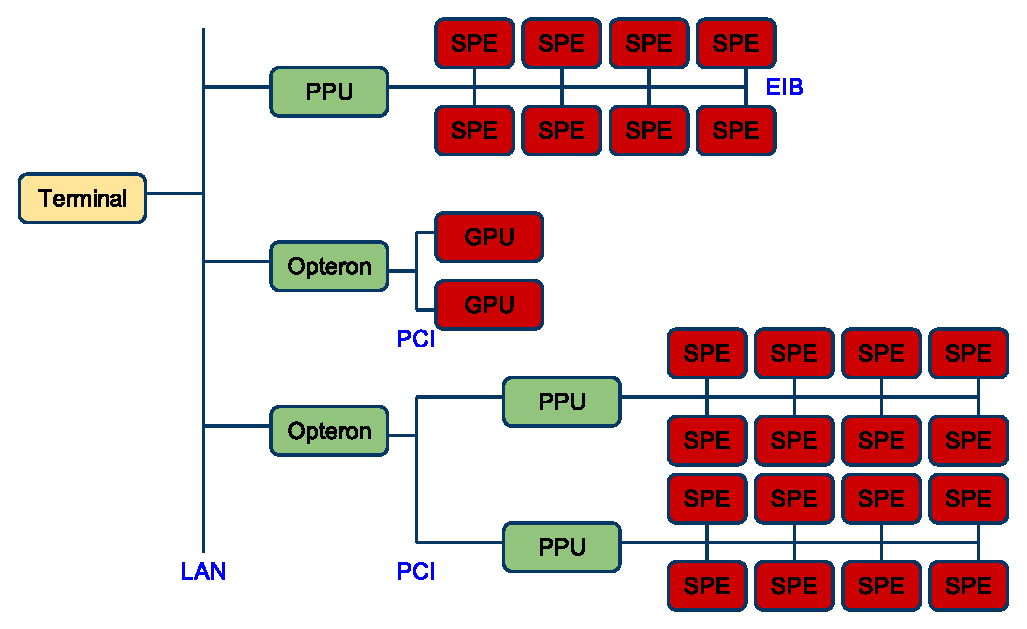
\includegraphics[width=3in, keepaspectratio]{hybrid-topology.eps}
\end{center}
\caption{Hybrid Topologies}
\label{fig:hybrid}
\end{figure}

Another recent trend is the rise of hybrid system and hybrid cluster
models.  Hybrid systems incorporate heterogeneous cores, either with
different processing characteristics or difference instruction set
architectures.  The Cell Processor, with its combination of a general
purpose PowerPC cores (PPU) and eight synergistic processing elements (SPE)
for vector operations is a classic example.  In such systems, the various
cores have coherent access to eachother's memory, but memory transfers
between PPU and SPE are handled explicitly.

A slightly more loosely coupled version of this can be seen in systems
using GPUs to accelerate compute.  In such systems, the GPU accelerators
are often located on the other side of a peripheral bus with their own
memory and execution units.  Existing runtime frameworks for GPUs, 
such as CUDA, provide preciously little introspection and control to the
external system -- making monitoring and control difficult.

The Road Runner tri-blades used a set of cell processors connected over
peripheral buses to a general purpose opteron combining both of the 
previous examples.  Road Runner poses many interesting challenges as
a Hybrid as it has multiple instruction sets, multiple endian, and multiple
peripheral buses.

These sorts of hybrid systems can themselves be composed together with
other more general purpose systems in a hybrid clusters.  The Virtual
PowerXcell Environment (VPE) was an attempt to create a runtime which
addressed such a loosely coupled hybrid cluster by trying to maintain
the illusion of a single system image.

\subsection*{Extreme Scale}

A final area of particular interest is extreme scale computing.
Blue Gene is capable of having hundreds of thousands of cores, with
subsequent versions aiming for millions.  Managing and debugging the
physical hardware at this scale presents a challenge, deploying, monitoring
and controlling application threads if even more daunting.
The lack of infrastructure capable of coping with this extreme scale,
has lead to oversimplified application frameworks only capable of statically
defined and managed embarassingly parallel applications.  We believe 
the development of a dynamic command and control framework for extreme
scale is the key to unlocking its true potential and broadening its
applications base.

Beyond sheer scale, systems such as Blue Gene present a number of 
interesting challenges for execution frameworks.  The machine employs
a physical paritioning mechanism to allow it to be used concurrently
by multiple users.  The physical partition scheme is limited by the
underlying machine architecture, creating a minimum allocation of one
I/O node and 64 compute nodes (at least at Argonne, smaller granularities
are possible, but the smallest is one I/O node to 8 compute nodes).
As a result, when requesting additional resources, you actually are
requesting a private cluster composed of some number of I/O nodes (which
are good for running certain types of tasks) and a certain number of
compute nodes (which are good for running another type of tasks).  This
complicates the cloud scenarios discussed earlier.

\begin{figure}[h]
\begin{center}
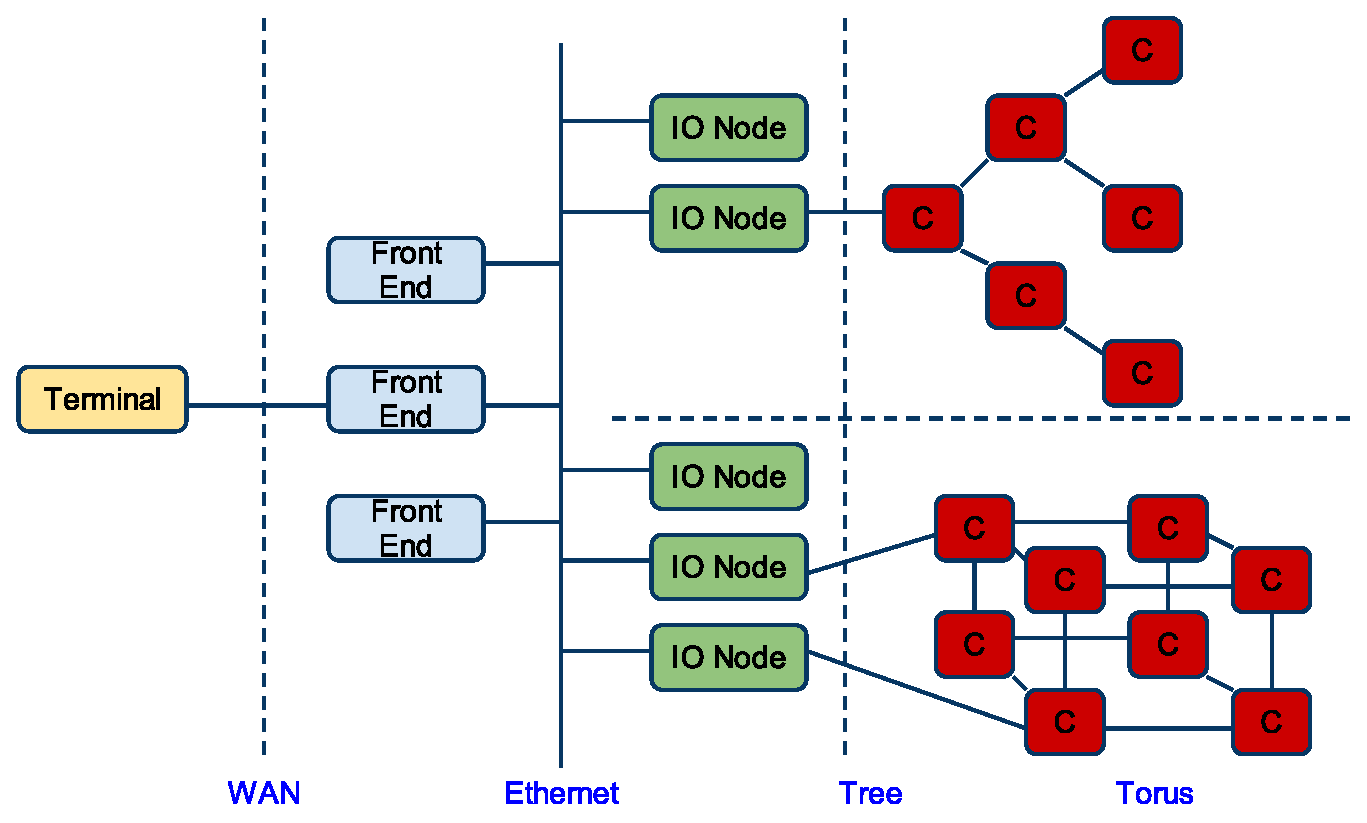
\includegraphics[width=3in, keepaspectratio]{bgp-topology.eps}
\end{center}
\caption{Extreme Scale Topologies}
\label{fig:bgp}
\end{figure}

Furthermore, extreme scale systems such as Blue Gene incorporate several
underlying physical network technologies which creates several different
network domains which cluster elements have to work within.  For example,
end-user workstations can only access the front-end nodes (which are
general purpose PowerPC servers).  The front-end servers can talk directly
to the management infrastructure as well as the IO Nodes, but not the
compute nodes.  The Compute Nodes can talk to the IO nodes over the tree
network, but not the high-bandwidth torus network.  Coordinating management
components (not to mention applications) in such a diverse topology is
challenging.

\section{Requirements}

While primarily intended as a research project, it is important that
whatever solution is developed is deployable in a number of contexts
including Linux, MacOSX, and Plan 9.  It needs to be able to support
Intel and PowerPC architectures (in 32 bit and 64 bit varietys) and it
is desirable that it incorporate support for accelerators such as GPUs
and SPUs.  It needs to be network agnostic, requiring only a reliable,
in-order tansport -- and it needs to support some forms of dynamic 
configuration and shouldn't require static configuration files to work.

% CLOUD

In order to accomodate cloud configurations, an execution model must not
only be able to initiate remote applications, but potentially to provision
new nodes to initiate remote applications on.  This essentially also implies
control of booting (and shutting down) system instances.  On clouds which
support it, it might also incorporate controls for migrating system
images (and contained applications) to new physical hardware.

Resource management software, such as load balancers will have to
monitor the currently allocated assets and know when to acquire more or
release existing resources in order to adapt to changing workloads.
Since the cloud environments have multiple network security domains, such 
an execution model will require mechanisms to be able to cope with 
traversing the multiple network spaces to maintain monitoring and control 
of remote processes. 

With so many different resources spread out across the cluster, users 
and applications will need new tools to be able to keep track of what
resources they are currently being charged for and how they are being
used.

Additionally, there are cases were it is desirable to run many instances
of an application on many remote nodes, breaking the original one-to-one
model of cpu(1).  We've seen this requirement take two forms: in one form
the important thing is just to start many duplicate copies of the application
with the same arguments and environment.  In such cases, it is the applications
responsibility to configure each instance appropriately.  Standard I/O in these
cases is primarily a logging mechanism as opposed to a mechanism for interaction
or reporting data.  The other case requires the ability to spawn off many 
instances, with individual configurations and control channels.  Finally,
while in most cases the applications are spawned from a single terminal or
front-end node -- we feel it is important that new instances (or resources)
may be allocated from within the cluster as well as from the front-end.

% HYBRID

For heterogeneous systems, we must have the ability to provision systems with
specific characteristics (ISA, Accelerator Properties, Memory, etc.) on
specific nodes.  We must also be able to accomodate infrastructures such as
CUDA which combine execution on the general-purpose CPU and the GPU 
accelerators.   As such, execution must be conditionalized on being able
to find sufficient resources to initiate execution.
In environments which support it, such as Cell, the execution model should 
provide controls to hybrid accelerator hardware.

Since hybrid models such as CUDA operate as black boxes, we must be able
to support dedicating hardware to a particular task as well as standard
time sharing models -- incorporating the same basic features as a 
cluster provisioning system such as cobalt or the sun-grid-engine at
a system image and/or task level.

Given that hybrid accelerators may be present over tightly coupled
peripheral buses (or even on chip) -- whever mechanisms are used to
establish command/control must be transport independent (ie. able to
run over a peripheral bus as well as over a standard IP network).

% EXTREME SCALE

In order to be able to use the execution model at systems with the
scale of Blue Gene (or potentially larger), the execution model interface
needs an organizational interface which can scale to millions of threads.
To be complete, it will have to handle physical resource provisioning at
multiple granularities (to match underlying cluster management tools) and
provide mechanisms to access hardware debug facilities.

Application threads at extreme scale often require extremely low latency
access to computational peers, adding the requirements of data locality
and physical topological awareness to any workload distribution and
management system.  Furthermore, it is likely that such applications will
require similar knowledge be integrated into whatever inter-thread
communication and synchronization primitives provided by the framework.

Application (and system image) deployment at large scale also provides
a challenging problem.  Some manner of aggregated deployment of application
images (and data) will be necessary in order to accomodate simulataneous
execution of thousands of new threads.

Furthermore, the overhead of monitoring such a large scale system 
is signifigant.  Any monitoring/reporting infrastructure will have to
be augmented so that the overheads of monitoring nodes does not overwhelm
their communication or computation capability.

Finally, the sheer number of components of such large scale systems make
failure of individual components more likely.  The systems infrastructure
for providing the execution model should be resilient in the face of
such errors, migrating workloads as appropriate and not failing itself when
it can no longer contact some of its components.

\section{Related Work}

Suffice to say, there have been a number of projects attempting to
address distributed execution models.  Within the space of the motivating
examples, the two most prominent paradigms are Map/Reduce and MPI
mechanisms -- both of which were designed with a particular application
structure in mind.  We seek a more general-purpose execution model
capable of handling the aforementioned requirements.

The XCPU runtime infrastructure was an attempt at bringing
the power of Plan 9's cpu(1) facility to HPC systems running
other operating systems.   It incorporated facilities for dealing
starting large numbers of threads on large numbers of nodes.  It
optimizes binary deployment using the treespawn mechanism which allows
it to task clients as servers to aggregate the work.  Its associated
monitoring infrastructure uses s-expressions to more easily allow
collection of correlated remote monitoring data from nodes.
The xcpu client also had provisions for supporting multi-architecture
hosts.

XCPU suffers from a rather ad-hoc authentication mechanism which isn't
persistent and ends up being a bit of a pain to deal with.  It doesn't
incorporate workload scheduling itself, relying instead on external
tools.  It also suffers from static configuration, and doesn't easily
support fanning out with individual arguments and I/O paths.  Finally,
XCPU's currently implementation is linked to scoket transports, and while
it supports the use of private namespaces and limited binding in XCPU2,
it only does so on modern Linux kernels.

There are a large number of process style interfaces both to local
processes and remote clusters.  These are summarized here for reference:
\subsection*{Plan 9 Proc Interface}
\begin{description}
\item[mem] the current memory image of the process
\item[proc] kernel per-process structure
\item[regs, fpregs, kregs] contain representations of user level registers
\item[fd] lists open file descriptors of the process
\item[ns] textual represntation of the process namespace
\item[segment] list of the memory segments associated with the process
\item[status] twelve field structure describing state of the process
\item[text] the file from which the process was executed
\item[wait] read to wait on children of the process and recover their exit message
\item[profile] contains instruction frequency profile information
\item[note] is used to send asynchronous notes to the process
\item[notepg] similar to note, but works on the whole process group
\item[noteid] contains the note group identifier of the process
\item[ctl] is used to control execution of the process, the following
messages are available
\begin{description}
\item[stop] suspend execution of the process
\item[start] resume execution of a stopped process
\item[waitstop] block the calling process until process is Stopped or exits.
\item[startstop] allow a stopped process to resume, and then do a waitstop action
\item[hang] set a bit in the process so that if it completes an exec system
call it will enter the stopped state before returning to user mode.  This bit
is inheritted across a fork
\item[closefiles] close all open file descriptors in the process
\item[nohang] clear the hang bit
\item[kill] kill the process the next time it crosses the user/kernel boundary
\item[pri] set the base priority for the process
\item[wire] set the affinity of a process to a particular core
\end{description}
\end{description}

\subsection*{Inferno Prog Interface}
\begin{description}
\item[status] semantically similar to the Plan 9 interface with different syntax
\item[pgrp] numeric identifier of the process group of a process
\item[nsgrp] numeric identifier of the namespace group of a process
\item[ns] similar to the Plan 9 interface
\item[wait] similar to the Plan 9 interface
\item[exceptions] give details of the last exception incurred by the process
\item[stack] contains dynamic call stack of the process
\item[heap] may be queried to examine the state of the process
\item[debugctl] debug control interface
\begin{description}
\item[step] step the interpreter for at most n instructions or until
a breakpoint is reached
\item[toret] step the interpreter until a return from the current activation frame or breakpoint is reached.
\item[cont] step the interpreter until a breakpoint is reached
\item[start] run the process ignoring breakpoints
\item[bpt set] set a breakpoint
\item[bpt del] delete a breakpoint
\item[stop] stop the process as soon as possible
\item[unstop] cancel the effects of the previous stop
\end{description}
\item[ctl] control the execution context with the following messages
\begin{description}
\item[kill] similar to Plan 9
\item[killgrp] kill every process in the process group
\item[restricted] mark all processes that this process spawns in the future as restricted.  Restricted processes are lmited in the amount of memory they can allocate such that they can't starve the entire system. 
\item[exceptions propagate] enables propagation of exceptions to children
\item[exceptions notifyleader] on exception, destroy all processes in the group except for the leader.
\end{description}
\end{description}

\subsection*{Inferno Cmd Interface}

The cmd(3) file system which provides an execution model for running
host threads on a hosted Inferno system, provides a directory per task
with control and status files as well as a files for stdin/stdout and
stderr.  It uses a top-level clone file, similar in operation to devip, 
which allocates new directories for new tasks.

\begin{description}
\item[data] can be read or written to get stdout or stdin respectively
\item[stderr] can be read to get standard error
\item[status] process statistics similar to Plan 9 and Inferno
\item[wait] can be read to wait on program to terminate
\item[ctl] used to control execution and accepts the following commands:
\begin{description}
\item[dir] sets working directory
\item[exec] execute a command with certain arguments
\item[kill] kill the host command immediately
\item[killonclose] set the device to kill the host command when the ctl file is closed
\item[nice] set process priority
\end{description}
\end{description}

\subsection*{Linux}

Linux has a great number of interfaces within its leaf proc directories.
Note that these files are mainly status or resource access with not command
and control files.
\begin{description}
\item[auxv] contains the contents of the ELF interpreter information
\item[cmdline] holds the complete command line for the process
\item[coredump filter] part of the core dump configuration
\item[cpuset] part of core affinity
\item[cwd] symbolic link to the current working directory of the process
\item[environ] environment variables of the process
\item[exec] symbolic link to the actual pathname of the executed command
\item[fd] subdirectory containing one entry for every file the process has open -- reading/writing these files reads or writes the underlying file descriptor
\item[fdinfo] subdirecotry containing one entry for every the process has open with information about the current status of the file descriptor.
\item[limits] specifies the per-process settings for various system imposed limits
\item[maps] a file containing the currently mapped memory regions and their access permissions
\item[mem] a file that can be opened in order to directly access a process' memory
\item[moutninfo] a file containing information abou the current mountpoint within the process
\item[mounts] a list of all file systems currently mounted in the process's namespace
\item[mountstats] this file exports statistics and configuration information for each mount within the namespace
\item[numa maps] NUMA information for the process (?)
\item[oom adj] can be used to adjust the score used to select which process is killed when the system runs out of memory
\item[oom score] the current score of the process with respect to its likelyhook of being killed during oom.
\item[root] symbolic link to the logical root of the proc's namespace
\item[smaps] shows the memory consumption for each of the proc's mappings
\item[stat] status information about the process (used by ps)
\item[statm] provides information about memory usage, measured in pages
\item[status] provides much the information of the stat and statm files in a format easier for human consumption
\item[task] a subdirectory which contains a subdirectory for each thread in a process
\end{description}

\subsection*{XCPU}

Another data point is xcpufs, which provides 10 file interfaces per thread,
as well as 5 top-level control files per node.  xcpufs provides its own files
for stdin, stdout, and stderr.  The top level files provide information on
the node (architecture, state, current processes) as well as files for
specifying default environments and namespace for tasks run on the host.
xcpufs also uses a clone file to allocate new tasks on a node.

xcpufs contains the following top level files:
\begin{description}
\item[arch] returns a description of the architecture of the host
\item[env] access to the environment under which the xcpufs server is running
\item[procs] list of proces (s-expressions?) running on this machine
\item[state] current state of the node
\end{description}
For every task, xcpufs contains these files:
\begin{description}
\item[argv] written to set argument list for current program
\item[exec] similar to Plan 9's text proc file
\item[env] local environment for this session
\item[fs] directory containing binary and all necessary additional files
pushed by the client
\item[stdin] pipe to standard in
\item[stdout] pipe to standard out
\item[stderr] pipe to standard error
\item[wait] returns the wait status of the running process on process termination
\item[id] session job id (similar to reading ctl on Plan 9 clone file systems)
\item[ctl] command and control file which accepts the following commands:
\begin{description}
\item[exec] execute the specified program within an optionally specified working directory
\item[clone] copy the complete dession directory to a remote node running xcpufs.  An optional number can be used to parameterize treespawning
\item[wipe] close standard I/O files for this session and send SIGTERM
\item[signal] send a signal to the running process
\item[type] specify whether the session is normal or persistent.  Persistent sessions remain until explicitly wiped, while normal sessions close then the control file is closed.
\item[id] set job id for this session
\end{description}
\end{description}

\subsection*{kvmfs}

Built by LANL, kvmfs provided a synthetic file system interface to 
control libvirt based hypervisors.

\begin{description}
\item[info] returns current memory and device information
\item[id] set to the user specified vm identifier
\item[fs] points to a directory containing temporary storage for a vm
\item[ctl] control file which accepts the following commands:
\begin{description}
\item[dev] specifices device image for a specific device (like a hard drive)
\item[net] create a network address with a specified mac
\item[loadvm] load vm state from a file
\item[storevm] stores the state of a vm to a file
\item[power] turn vm power on or off
\item[freeze] suspend execution of a vm
\item[unfreeze] resume execution of a vm
\item[clone] creates copies of a vm (in a fashion similar to xcpu clone)
\end{description}
\end{description}

\subsection*{BGDBFS}

{BGDBFS} was a synthetic file representation of the cluster JTAG mechanisms
available on Blue Gene/L which we used in order to bring-up Plan 9 on the
system.  Physical nodes were addressed within a allocated partition (aka bump)
and addressed by a node number (and optionally a core number).  This
addressing formed the top level directory of bgdbfs (one bgdbfs instance
per bump).  While we originally supported individual access to both cores, 
we fell back to a simplified model only dealing with the first core as we
didn't have SMP support for BG/L at the time.  We had a more interactive
console at one point, but abuse by certain project members (which would lead
to problems with the hardware) forced us to fall back to a non-interactive
log mechanism.

\begin{description}
\item[log] non-blocking console log
\item[sprs] dump special purpose registers
\item[msr] dump machine state register
\item[iar] instruction address register
\item[torus] torus device register dump
\item[tree] tree device register dump
\item[info] per node personality information dump
\item[cpu] executable syntheticly generated script to get to node
\item[status] node status
\item[fpregs] floating point registers
\item[mem] physical memory of node
\item[proc] unimplimented
\item[regs] general purpose registers on node
\item[text] kernel image (unimplemented)
\item[ctl] control interface accepting the following commands:
\begin{description}
\item[kill] terminate execution of entire partition
\item[start] resume core execution
\item[stop] halt core execution
\item[startstop] single step core execution
\item[reboot] reboot the entire partition
\item[allocate] allocate a block partition
\item[boot] boot an allocated partition
\item[resetimage] return image configuration to system default
\item[9image] configure image to be the Plan 9 boot image
\item[free] release the allocation of a partition block
\item[reset] attempt to reinitialize access to jtag interface
\end{description}
\end{description}

While there is plenty of overlap in these various interfaces, there are
obvious differences -- some without much logical reason.  It is imperitive
that common features have common interface syntax and semantics to maximize
familiarity among the user base.

\section{Design}

The core idea is to build upon the ideas present in xcpu, xcpu2, and
to some extent spufs, cellfs and kvmfs to provide a comprehensive
execution model which covers allocation and management of logical 
nodes as well as distributed execution and to some extent communication.  
The idea is that this could provide a more dynamic execution
model for EC2 deployments of Plan 9 and Inferno as well as 
provide the foundation for large scale deployments of applications
as part of the DOE HARE project.  This should also fill the distributed
execution requirements for the PUSH project (which in turn will provide
facilities for connecting distributed execution in a pipeline fashion).

%a scope-driven hierarchy (a level for logical nodes, a level beneath
%that for processes on those nodes (perhaps several different classes
%of levels beneath logical nodes representing different types of thread
%(limbo, native host, or emulated).  The idea would be the same
%interface for local, remote, or hosted (in the case of Inferno) (or
%emulated in the case of CNK on BG/P).  Push could then interact
%directly with this hiearchy to deploy threads.  Another side-aspect is
%alternate views -- the hierarchical layout is the canonical form, but
%there may be other views which can be obtained which make more logical
%sense (ie. nodes/threads associated with a user, a task, or whatnot),
%the other "requirement" would be for some sort of cluster-based
%allocation as opposed to just individual node (ie. start up 100 nodes,
%each running 4 threads of this executable).  While this could be
%incorporated into the ctl interface (as it is on xcpu to some extent),
%it might be nice to be able to do such an operation in a cluster view,
%but then be able to access the individual threads in the user-view or
%the canonical view.

The core interface principle remains as a service-oriented file system
based on the same basic design as proc(3) or Inferno's prog(3).  
The idea, is at its core, each thread will have its own directory with a 
number of control files.  

The basic design builds upon these past designs by using clone files to
allocate new resources in much the same fashion as the cmd device from Inferno
or xcpufs.  Each newly allocated resource will have a subdirectory
containing control/status files specific to the resource which the directory 
represents.  Certain standard files are provided at every level 
(for instance ctl and status) -- but the semantics/syntax of interacting with 
them may be more specific to the underlying resource.

The use of clone files to instantiate threads may be a bit controversial
as it always comes up as the example of how we don't want to use a file
system for everything.  However, I believe the need for distributed
execution contexts trumps prior reasons for not instantiating new threads
through a file system interface.  Its not clear that there should be a
complete switchover to using file system operations for things such as
fork, but it seems clear that we need an architected mechanism for 
execution in other contexts.  By using a synthetic file system for
this interface, it means we can easily export it to other environments --
all the system would need is a 9P client library or file system in order
to access the execution model.

For example -- Inferno and Plan 9 have different files based on what
underlying information and controls are avaialble.  Given the wide 
space we intend to address, this will likely be the case for us as well.

% Organization
The sheer number of nodes and threads we intend to support will not
be possible with a flat organizational structure.  One approach would be
to use a hierarchical structure matching the physical organization of the
nodes 
(ie. data center $\rightarrow$ row $\rightarrow$ rack $\rightarrow$ chassis $\rightarrow$ slot $\rightarrow$ lpar $\rightarrow$ thread 
for a blade configuration).  Such a model might have multiple clone files at
multiple levels providing abilities to intantiate new logical nodes, logical
partitions, or threads.
Another model would be to match the logical organization
of a cluster management tool (i.e. job number $\rightarrow$ IO Node $\rightarrow$ CPU Node $\rightarrow$ Core or Thread
for Blue Gene).  A similar model would be possible for Cloud 
configurations.  
Another related model would be to use network topology in order to address
resources.  This would provide semantic information in order to directly
contact or allocate neighbors in a torus or other locality based 
topology.

Perhaps the most flexible approach would be to allow users to define an
arbitrary hierarchical organizational structure using a /n-like dynamically
generated organization terminated by a clone file to allocate resources at
that level of the hierarchy.  In cloud configurations, such a dynamic 
hierarchy could also be used to help allocate machines with specific 
attributes (i.e. $/cloud/x86/gpus=1/mem=4G/clone$).  The same technique
could be a general mechanism to find hardware capable of supporting the
objtype of a given application (or allocating the hardware as necessary).
There should be a relative mechanism available which chooses reasonable
defaults based on the currently executing application such that a user
doesn't have to specify an exhaustive list of attributes for every 
innvocation.

The likely case is that any chosen organizational structure will not be
optimal for every type of access.   That is to say, one organization will
not be sufficient.  As such, it is desirable to provide multiple views into
the model: supporting physical, logical, and user-defined views.  This should
be possible through the use of a generic key/value tagging facility which
should provide sufficient flexibility to satisfy most constraints.
This same solution should be able to work with both physical resources
as well as user-defined tasks and logical resources.

Another parameter which might be useful in such organizations is to
provide scoped dynamic attribute specified access.  That is to say, provide
a subdirectory which when traversed will perform resource lookup based
on the scope of the current level of the hierarchy.  This could be used
to find a node within the current logical group which has a certain
resource available, or be used to provide flat access to all processes
within the current logical group.

Finding a mechanism to be able to switch between these alternate views
of the unified execution model will be critical.  A shortcut mechanism
such as dot-dot-dot may be appropriate here.

Due to the variety of underlying resources, it is desirable to 
provide a plug-in interface for both the organizational structure of
the execution model as well as the thread-level elements for different
back-ends.  This will allow for new resources to be added to the model
with a minimum of fuss, and allow for easy construction of unforseen
organizational structures.

An vital design element is that the unified execution model is not
a centralized resource.  Each element of the system which can will run
their own instance of the synethetic service-oriented file system.  These
instances will coordinate with one another in a fashion appropriate to
their underlying network topology.  Since many nodes will never have
to contact one another, cross-mounts are lazy and initiated on access.

This approach implies that every client is also a server.  Since we 
want to be able to traverse network boundries such as firewalls, NAT
appliances, and bridges between different network technologies it is
important that we are able to use a single connection for the two nodes
to be able to access eachothers resources and provide mechanisms for
nodes to be able to transitively access eachother through bridge nodes.
In the future, these relationships will be managed by retooling the
srv(3) mechanisms to be more cluster aware -- but in the short term we
can experiment with these different methodologies directly within the
execution model.

Aggregated data access is a critical element of the execution model in
order to be able to cope with scale.  It will be unacceptable to issue
millions of directory traversals and individual file operations in order 
to obtain a snapshot of the cluster's state.  As such, directory data must
be available in a compressed alternate form such as the s-expressions 
employed by xcpufs. 

\subsection*{Semantic File Systems}

TODO: Describe the semantic file system mechansim in more detail.

TODO: Talk about generic methodologies behind user and system defined 
tagging and key--value pairs.

TODO: also discuss how semantic file systems can be used for various
monitoring and management functions.

\subsection*{Multidimensional File Systems and dot--dot--dot}

TODO: Describe multi-dimensional file systems and the dot--dot--dot 
shortcut mechanism to more easily change views while maintaining context.

\subsection*{Canonical Reference Views}

Discuss the concept of a canonical reference dimension and how it can
be used to short-circuit transitive references creating more efficient
pipelines and potentially file systems.

\section{Implementation}

Hosted Inferno seems a natural choice to implement these designs.  It already
has its own authentication mechanism and full dynamic private namespace
facilities.  It runs on all target operating systems and provides a nice
abstraction of their underlying differences.  Furthermore, through the cmd(3) 
infrastructure it is able to initiate and control processes on the 
underlying system.  
An interesting aspect of this setup is that we can start both Inferno threads
or host threads using roughly the same interface -- that can be extended to
initiation of CUDA threads and/or emulated environments (such as linuxemu
on Plan 9 or cnkemu on BG/P Plan 9).
These threads can access resources such as the 
initiating nodes file system through a 9P backmount which can be organized
and exported via Inferno (MacOSX will have to use FUSE to do the back-mount,
but this allows us an Inferno pseudo-dynamic-private namespace on OSX).

Additionally, the general idea is for Inferno to export the synthetic
file system interface of the exection model to the underlying host allowing
it to directly access the interfaces and initiate actions either via shell
scripts of library APIs.  This is why it is of vital important that all
interaction should be possible using only the file system based interface.

A potential gap is that Inferno does not currently support .U extensions
necessary for some Linux applications.  We'll need to look into mechanisms
for either implementing .U semantics within Inferno or bridging them to
remote servers which implement them.

While Inferno may seem a bit heavy weight for this task, consider that the
text size of many comparable infrastructures is far greater.  Even
XCPU isn't that much smaller than a full blown Inferno execution.  In the
future this overhead may be further diminished by creating an
Inferno stand-alone-complex for the execution model which eliminates the
virtual machine and graphical components of the hosted inferno emulator.
The working term I've been using for such a stripped environment is the
Basic Resource Aggregation System Inferno Layer (aka Brasil).

Limbo's dynamic module loading seems to be a fairly optimal solution for the
integration of plugins.  A file based interface (perhaps even a plumbed one)
can be used to instruct the execution model to load new plugins dynamically --
relying on a static configuration to load the defaults for a particular
system (and/or user).

It seems clear that there are at least two different forms of plugins: 
back-ends which supports allocation, execution, monitoring, and control of
specific physical or logical resources (clusters, nodes, logical partitions,
threads, accelerators, etc.) and front-ends which support different
organizational models (physical hierarchy, logical hierarchy, attribute
based search, task-based, etc.).  The existence of different underlying
transport mechanisms may require plugin support as well -- but it is less
clear to me how that can be easily integrated and may be best left to a
separate infrastructure (such as /net or /srv).

Back-end plugins will provide two levels of directories -- a toplevel which
is the same for each physical instance of the resource group, and an 
instance directory with the per-instance control and status interfaces.
These two level directories can be stacked (such that per-instance directories
might contain another resource's toplevel and instance subdirectories).  This
allows compositional hierarchies to be easily built.  TODO: figure out syntax 
of how this is going to play out via the file system or modular interface.

Access to compressed aggregated information about a subset of the
resources will be made available through an alternate attach point of the
synthetic file system (and optionally through a dot-dot-dot shortcut).

Communication and coordination of different instances of the execution
model will be accomplished via a single pipe.  Client and Server messages
will be sent on the same pipe, with a special mux on either end capable of
distributing requests or responses as appropriate.  This will allow
communication between two hosts when only one of the hosts is addressable,
it will also allow easier tunneling of communication paths.  Extensions on
this mux to allow bridging of network domains will also have to be investigated.

The essential idea is that each participant in the unified environment will
run their own instance of the execution model.  They will communicate directly
with that instance in order to interact with other nodes (through their
instances).  In other words, every thread talks to its local instance, and
the instances are responsible for coordinating with eachother.  This keeps
the model decentralized and should allow for enhanced latencies when dealing
with local resources versus remote resources.



\section{Examples}

In order to validate the interfaces described above, I'd like to run through
a few scenarios of user or application interaction with Brasil.

\subsection*{Kirin Hybrid Cluster}

The first use case we will explore is the use of this mechanism within our
KIRIN cluster, which is a set of opteron workstations running Linux  with 
GPU peripherals and CUDA runtimes.  We want to be able to allocate machines
(and GPUs) to run distributed applications on, and have some rudimentary
communication mechanisms for control of the threads of the application as well
as a communications channel for communicating results back to the initiating
host as segments of computation complete.  In our case, the initiating host
is a Mac Pro laptop running its own instance of CUDA in order to visualize
the results of the computation.

For the purposes of this example, lets say our application is a computational
intensive imaging application.  The image to be processed is a large file on
the disk of the initiating host.  The front-end application is setup to 
split up the image into uniform tiles and provide the tiles to the distributed
worker threads to process and return the processed tile back to the initiating
host.

The master thread parses the image file to a sufficent degree in order to
determine an upper bound on the number of logical instances which would be
required to process the image completely in parallel.  The user, either
by parameter, configuration file, or environment may limit the maximum
number of requested logical gpu instances.  It then requests reservation of 
that many GPU instances across the cluster and initiates execution of
subject threads built using the CUDA runtimes.  These subject threads then
block on reading their standard-in to request work.  The master thread, who
has references to the stdin, stdout, and stderr of each subject thread instance
issues work assignments by sending a relative path to the master file along 
with coordinates specifying the tile that the thread in question is instructed
to process.  It is important to note here that, following the xcpu2 model, the
subject threads have the same file system namespace as the initiating thread.  
As threads complete their assigned work, they can either write
an image file of their own to the shared file system or send the results over
standard out directly to the master thread.  Upon receiving results, the
master thread can issue more work, or instruct the subject thread to terminate
and release the resource.

\begin{figure}[h]
\begin{center}
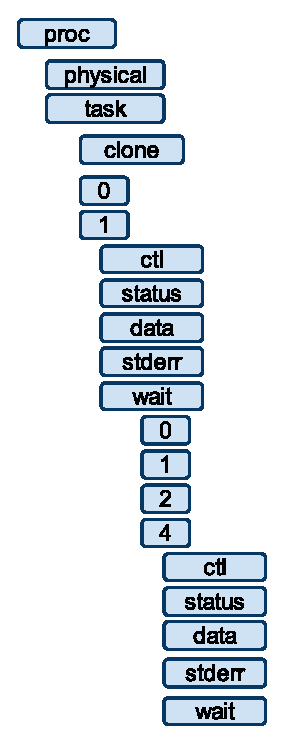
\includegraphics[width=1in, keepaspectratio]{kirin-proc.eps}
\end{center}
\caption{Kirin Task Example}
\label{fig:kirin}
\end{figure}

The master thread can coordinate this activity and communication directly 
using the synthetic file system, but it is much more likely that it will do
so via a simple library API.  Specialized versions of this library can be
constructed for certain classes of application and provide more advanced
facilities such as Cilk-like work stealing, data pipelining between 
computational elements (ala PUSH), or transactional semantics enabling 
either checkpoint/restart or triple modular redundancy of computation.
Eventually, it would be nice to incorporate these facilities into runtimes
which manage issues involving different instruction set architectures.

From an implementation perspective, we really have two different organizational
elements: physical resource allocation and task based execution.  The first
thing we need to do is allocate some number of GPU nodes where the maximum
is defined by user specification or the actual available resources.  There
is not really an existing example mechanism which allows us to allocate a
group of physical resources without logical sharing or blocking.  We could
query existing available resources and then dispatch tasks using the clone
mechanism -- but there is an inherent race condition between the checking of
the resources and the dispatch of children.

A strawman approach is to use a task-based organization -- the master thread
opens the clone file on the task view of the execution model.  This clone file
creates a new task session id, and creates a subdirectory with that session id.
Subsequent reads and writes to the fd which was opened as the clone file will be
directed to the ctl file of that subdirectory following the typical clone
semantic of Plan 9. 

For the purposes of this strawman, lets say his image has 100 tiles to process.  He issues a command to reserve 100 GPUs, and gets an error response that 
only 4 GPUs are available.  
He re-issues the request asking for 8 GPUs, which succeeds.
This creates 8 new subdirectories in the task session directory, each 
representing a thread on the local or remote system which has been allocated
a GPU resource.
Since he is executing the same subject thread on the resources he can use
his existing fd handle to issue the execute command to all subject threads.
The master thread can then open the data file of each subdirectory in order
to obtain a communications handle to the remote threads on which he can
issue work assignments and read results (or pointers to results).

When finished, he can cleanup the allocated resources by closing the handle
to the ctl file.  Individual threads can be shutdown or retasked by opening
their individual ctl files present in the subject thread subdirectories.
  
\subsection*{BG/P Allocation and Debug}

On more of an infrastructure focus, I'd like to use the unified execution
model to be able to allocate resources and provide hooks to debug the 
kernel using either JTAG hardware (for BG/P) or hooks in the hypervisor (for
Cloud).  As mentioned earlier, Blue Gene presents an interesting problem
in that physical partitions of the machine have to be allocated at some fixed
granularity (such as 1 IO node and 64 compute nodes on the BG/P at ANL).
Another interesting factor is that physical machine allocations are handled
by a batch-job allocator underneath.
So, we need to be able to cope with group allocations of multiple granularities,
and must be prepared for waiting for extended period of times while the
parition is allocated or resources for that size partition become available.

A model similar to the resource reservation methods described in the Kirin
cluster should allow us to request various physical partition sizes and
characteristics.  Instead of failing when resources aren't available, an
option to the reservation can choose to block the request until resources
become available.  Since Blue Gene can be configured to boot different
kernel images, the reservation mechanism can specify alternate kernel 
profiles and/or parameterization to the various kernels.  Configuration
commands needs to be set prior to issuing the reservation command.

The top level control file can be used to issue commands to Cobalt
(such as terminating an allocation) and can also be used to query both
the status of our task and obtaining the status of other runs on the
machine and direct access to various machine log files.

The hierarchical nature of Blue Gene's physical topology creates another
interesting difference.  When the reservation successfully completes, the
top level session directories will be for the IO nodes for a particular
logical partition.   The compute nodes accessible via that IO node will be
represented in session directories under the IO node's session directory.

For Blue Gene we are interested in both remote command execution and
physical node access and debug.  As such, in addition to the normal execution
control and status files in the IO node and Compute Node directories, we'll
also provide top-level debug and memory access.  Since each of the cores on
a BG/P have separate hardware registers, we'll provide access to the per-core
registers in subdirectories.  Since the normal session syntax uses numbers
which will relate to processes executing on that node, we'll use alphabetically
identifiers (A, B, C, D) for the various cores.  Debug commands issued to the
ctl file in the core subdirectories will only effect that core, while debug
commands issued at the top level will effect the entire node.

While initiating tasks from the physical hierarchy view can be useful, it is
much more likely we'll want other configurations for starting new tasks.
One possibility is the desire to start a task on a neighbor node in the
torus.  In order to do this, we'll need to provide an alternate organizational
topology for the node session access which takes the form of the Torus's
three dimensional configuration.  This can provided in an alternate attach
namespace reachable from the partition's top-level or through a dot-dot-dot
shortcut. Beyond physical or network topology, it may be desirable to provide
user allocated node groupings, this will be accomplished through a new special
session control file named tag which will be present at all levels of the
hierarchy and can be used to apply new tags to individual nodes or nodes and
their children.  Access to nodes using these tags can be done through a 
semantic search hierarchy also accessible from the top level of the 
partition session directory.

So, to execute a Monte Carlo simulation on a BG/P, the Master Thread of
the application needs to first request a BG/P partition of the appropriate
size (lets say 512 nodes).  If that size allocation is not immediately
available, it returns an error, and the master thread re-requests the
512 nodes with an option which blocks the read until the resources become
available.  Once the resources become available, the read unblocks.

The user sets up the Monte Carlo thread execution on all available
cores passing parameters via stdin just like in the Kirin example.
For the sake of the example, lets say some of the Monte Carlo threads
have a state where they need to spawn off additional simulations with
slightly different parameters to complete their simulation.  When these
threads reach this state, they can initiate thread execution using their
local instance of the unified execution model.  It will find nodes that
have either already completed their simulation or those who have a lower
load average and schedule the new threads there.  Alternatively, the user
can provide parameters specifying they want the execution to completely closer
to the initiating thread and the execution model will try to schedule the
thread on the same node, or on a node which is located closer from a network
point of view.

\section{Discussion}

The examples in the prior section map out a set of experiments to explore
various interface and interaction models for the unified execution model.
They are not intended to provide a complete set detailing the scope of its
functionality, but serve as a jumping off point to evaluate and extend
the ideas.

TODO: There's lots of gaps to be filled in and the blue gene example needs more
illustrations and a more complete walkthrough.

Another thing we didn't talk about at all as how this relates to the
aggregation infrastructure discussed in the MTAGS paper.

\section{Acknowledgements}

This work has been supported by the Department of Energy Of Office of 
Science Operating and Runtime Systems for Extreme Scale Scientific 
Computation project under contract \#DE-FG02-08ER25851.

%
% The following two commands are all you need in the
% initial runs of your .tex file to
% produce the bibliography for the citations in your paper.
%\bibliographystyle{abbrv}
%\bibliography{brasil} % sigproc.bib is the name of the Bibliography in this case
\end{document}
